% ======================================================================================
% CLUSTERING
%
% graphs to insert:
%	- score vs silhouette coefficient per cluster
%	- sample silhouette values for the best number of clusters
%	- 3D/2D cluster representation for the best number of clusters
% tables to insert:
%	- PCA outcome of the features
%	- object to cluster assignment depending on number of clusters (the best ones)
%	- cluster sizes depending on number of clusters
% figures:
%	- mean values of the features per cluster applied to the object


\section{Clustering}

\subsection{PCA}

\begin{table}
	\begin{tabular}{ c c c c c }
		\hline
		\multicolumn{5}{c}{Principal Components} \\ \hline
		-0.51661962 & -0.51137137 &  0.59560332 &  0.29608388 &  0.17086402 \\ \hline
		-0.36102909 &  0.33317829 & -0.15354445 & -0.22331964 &  0.82776969 \\ \hline
		-0.07275141 & -0.28151638 &  0.19427207 & -0.92743392 & -0.13259127 \\ \hline
	\end{tabular}
	\caption{Principal axes in feature space, representing the directions of maximum variance in the data. We can see that the features 3, 5 and 4 the most variant ones.}
	\label{tab:pca_components}
\end{table}

\begin{table}
	\begin{center}
		\begin{tabular}{cc}
			\hline
			Variance & Ratio \\ \hline
			1.9754988 & 0.39498577 \\
			1.12242609 & 0.22442045 \\
			0.89518261 & 0.17898487 \\
			\hline
		\end{tabular}
		\caption{Variance and their ratio for the principal features.}
		\label{tab:pca_variance}
	\end{center}
\end{table}

PCA was performed to keep the three most variant features of the samples. In \ref{tab:pca_components} we can see the principle axes for maximum variance in the data. From this we find that the features that vary the most are in order of variance 3, 5 and 4 that correspond to: ratio between area of grasp and area of object, direction of vector between center of grasp and center of object in y-axis, and the direction of this same vector in the x-axis. In \ref{tab:pca_variance} we can see the variance for each of these three features as well as their ratio for the dataset.

In total these features represent around 80\% of the entire variance, seeing how we have five in total, this would mean that the other two would represent around 10\% each which is of quite small significance compared to the other three, we therefore can be content about this new dimensional reduction.


\subsection{K-means}

\begin{figure}
	\begin{subfigure}[b]{\textwidth}
		\input{plot_clustering__mean-silhouette}
		\caption{Mean silhouette coefficient per number of clusters.}
	\end{subfigure}
	\begin{subfigure}[b]{\textwidth}
		\input{plot_clustering__sum-sqr-dist}
		\caption{Sum of squared distances per sample to their closest cluster by number of clusters. Used in the \texttt{elbow method}.}
	\end{subfigure}
	\caption{Mean silhouette coefficient and sum of squared distances per sample to their closest cluster, depending on number of clusters. \texttt{best fit} identifies the possible best number of clusters in accordance to the maximum value of the mean silhouette coefficient and the elbow method.}
	\label{fig:kmeans_score}
\end{figure}

\begin{figure}
	\begin{subfigure}[b]{\textwidth}
		\input{plot_silhouette_5}
		\caption{Silhouette coefficient per samples for five clusters.}
	\end{subfigure}
	\begin{subfigure}[b]{\textwidth}
		\input{plot_silhouette_6}
		\caption{Silhouette coefficient per samples for six clusters.}
		\label{fig:silhouette_6}
	\end{subfigure}
\end{figure}
\begin{figure}
	\ContinuedFloat
	\begin{subfigure}[b]{\textwidth}
		\input{plot_silhouette_7}
		\caption{Silhouette coefficient per samples for seven clusters.}
	\end{subfigure}
	\caption{Silhouette coefficient per sample in each cluster for five, six and seven number of clusters.}
	\label{fig:silhouette_coef}
\end{figure}

\begin{figure}
	\begin{subfigure}[b]{\textwidth}
		\input{plot_clustering__clusters-2d}
		\caption{Two-dimensional representation of the samples and their assigned clusters and centroids.}
	\end{subfigure}
	\begin{subfigure}[b]{\textwidth}
		\input{plot_clustering__clusters-3d}
		\caption{Three-dimensional representation of the samples and their assigned clusters and centroids.}
	\end{subfigure}
	\caption{A two-dimensional and three-dimensional representation of the sample space with their assigned clusters and centroids for six clusters.}
	\label{fig:clusters}
\end{figure}

K-means was later run on the transformed data for a number of output clusters ranging between two to fifteen. As to choose the best fit of number of clusters we later look at the mean silhouette coefficient and the sum of squared distances from each sample to their closest cluster center. These results are presented in \ref{fig:kmeans_score}. By using the \texttt{elbow method} on the graph containing the sum of squared distances for the samples, we can judge that a number of clusters between five and eight is suitable. With the help of the silhouette score, where six clusters give the best results and falls into this range, we can conclude that six clusters is our best fit.

Figure \ref{fig:silhouette_coef} shows us the silhouette coefficient per sample for the three cases of five, six and seven clusters. We can see that for five clusters there are a lot of samples that have a very poor coefficient in some clusters. Seven has a better repartition but the gradient is quite important for the larger clusters. While six gives us something more balanced, and thus confirming it is a better choice.

Figure \ref{fig:clusters} show us a two-dimensional and three-dimensional representation of the data divided into clusters and their centers for six clusters. We can notice that it is not entirely obvious how the data is clustered as the data is a bit hard to reduce in dimensionality and visually represent in graphs. However the results for the silhouette scores and elbow method do confirm this clustering.


\subsection{Object cluster assignments}

\begin{figure}
	\input{plot_clustering__obj-sampl-assgmnt}
	\caption{Heatmap over distribution of object samples between clusters.}
	\label{fig:obj_sample_heatmap}
\end{figure}

\begin{table}
	\begin{tabular}{|c|l|}
		\hline
		Cluster & Objects \\
		\hline
		one   & hammer, pen, scalpell, scissors, knife, screwdriver, brush \\
		two   & box \\
		three & - \\
		four  & can, pitcher, glass, bottle, cup \\
		five  & tube \\
		six   & cutters \\
		\hline
	\end{tabular}
	\caption{Cluster assignment of objects between six clusters.}
	\label{tab:object_cluster_assign}
\end{table}

\begin{figure}
	\centering
	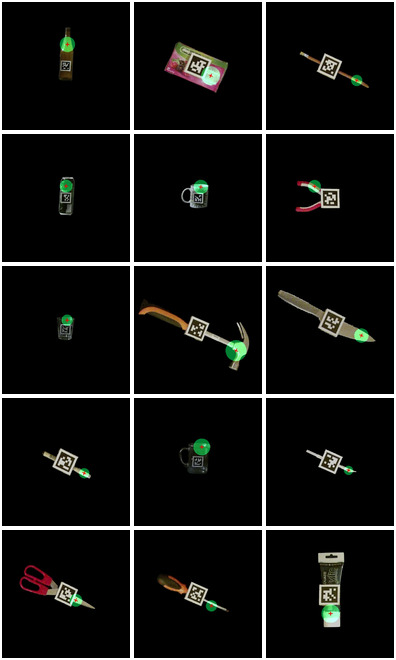
\includegraphics[width=\textwidth]{img/results/objects.jpg}
	\caption{The training objects with the mean values of the corresponding cluster applied to them.}
	\label{fig:results_objects}
\end{figure}

In figure \ref{fig:silhouette_6} we observe two dominant clusters, the first and fourth one. Figure \ref{fig:obj_sample_heatmap} represents a heatmap over the distribution of samples belonging to each object between the clusters. We can see that each cluster represents at least one object, with the exception of the third cluster. The screwdriver, knife, scissors, pen, hammer, scalpell and brush have the largest majority of their samples belonging to the first cluster, while the bottle, pitcher, glass, cup and can are represented by the fourth cluster. The cutters, box and tube are represented by their own clusters, respectively sixth, second and fifth clusters, showing that they are handed over in unique ways compared to the other previous objects. The third cluster seems quite evenly distributed over the objects, with the pitcher having the larges part, which indicates that it can be considered as a cluster of noise from the input data. Table \ref{tab:object_cluster_assign} shows us the final distribution of the objects between the clusters. In figure \ref{fig:results_objects} every object is visualized with their corresponding cluster mean features applied to them.

Already here we can see some similarities between the objects that are clustered together, notable in clusters one and four. The first one includes objects that are longer and thinner and that often include a tip of contact for it's usage, like the head of the hammer or the tip of the brush. While the fourth cluster is made of objects that are larger and cylindrical, often used for containing fluids which explains they need to be held similar fashion when handed over as to not spill out the contents.



% ======================================================================================
% CLASSIFICATION
%
% GRAPHS:
%	- loss per step
%	- accuracy per step (validation and testing)
%	- training speed
% TABLES:
%	- confusion matrix
%	- accuracy per object
%	-

\section{Classification}

\subsection{Network configuration}
\label{sec:res_setup}

To summarize the clustering part of this work we are able to divide the objects used for training into a total of five classes. An issue with these results is that three of the classes are represented by a sole item. We judge that it would not be possible to create a balanced dataset to represent equally each class this way. It would also defeat the purpose as to create a model that no longer identifies single object classes, but instead visually similar objects within a same class. Therefore we will discard these three classes and concentrate on the two classes that contain multiple objects. Our network will then be trained for two outputs.

\begin{table}
	\begin{tabular}{|c|p{5cm}|p{5cm}|}
		\hline
		Class & Training objects & Test objects \\
		\hline
		one & hammer, pen, scalpell, scissors, knife, screwdriver, brush & scissors, fork, knife, spoon, spatula, wooden spoon \\
		\hline
		two & can, pitcher, glass, bottle, cup & bottle, carafe, glass, cup, wine glass, beer glass \\
		\hline
	\end{tabular}
	\caption{Overview of objects included in training set and test set.}
	\label{tab:classification_objects}
\end{table}

In section \ref{sec:testing} we gave a list of objects that are to be used for testing. These were chosen after we made the decision regarding outputs for the network to achieve a balanced dataset over the outputs for testing. Table \ref{tab:classification_objects} shows the distribution of the test objects into classes with the corresponding training objects.


\subsection{Initial testing of batch sizes and learning rates}

\begin{figure}
	\begin{subfigure}[b]{\textwidth}
		\input{plot_classification__learning-rates__loss}
		\caption{Loss.}
	\end{subfigure}

	\begin{subfigure}[b]{\textwidth}
		\input{plot_classification__learning-rates__val-acc}
		\caption{Validation accuracy.}
	\end{subfigure}
\end{figure}

\begin{figure}
	\ContinuedFloat
	\begin{subfigure}[b]{\textwidth}
		\input{plot_classification__learning-rates__test-acc}
		\caption{Test accuracy.}
	\end{subfigure}
	\caption{Loss, validation and test accuracy for batch size 32 and different learning rates.}
	\label{fig:res_init_lr}
\end{figure}


\begin{figure}
	\begin{subfigure}[b]{\textwidth}
		\input{plot_classification__batch-sizes__loss}
		\caption{Loss.}
	\end{subfigure}

	\begin{subfigure}[b]{\textwidth}
		\input{plot_classification__batch-sizes__val-acc}
		\caption{Validation accuracy.}
	\end{subfigure}
\end{figure}

\begin{figure}
	\ContinuedFloat
	\begin{subfigure}[b]{\textwidth}
		\input{plot_classification__batch-sizes__test-acc}
		\caption{Test accuracy.}
	\end{subfigure}
	\caption{Loss, validation and test accuracy for learning rate 1e-05 and different batch sizes.}
	\label{fig:res_init_bs}
\end{figure}


In a first attempt to finetune the network to our data some training sessions are performed as to consider within what range the training parameters' optimal values lie within. Initial tests for finetuning the network are presented in figures \ref{fig:res_init_lr} and \ref{fig:res_init_bs} where we do coarse testing for which batch size and learning rates are optimal. With these results we will later try parameters within a smaller range to conclude which are their optimal values. All training sessions were performed with a K-fold cross validation of five and trained for a total of 20 epochs with a dropout value of \(0.5\). The figures show us the loss, validation and test accuracy at different learning rates of \([0.1, 0.01, 0.001, 0.0001, 1e-05]\) with a fixed batch size of \(32\) (figure \ref{fig:res_init_lr}) and different batch sizes of \([128, 64, 32, 16, 8]\) with a fixed learning rate of \(1e-05\) (figure \ref{fig:res_init_bs}).

First observations of the results in \ref{fig:res_init_lr} indicate that learning rates larger than 0.0001 make the network unable to learn from the data, probably as a result from the learning rate being too large for descending the local minima. This is confirmed by how training with the smallest learning rate, 1e-05, is the one that performs the best on test and validation accuracy.

By inspecting the results of differently sized batches in \ref{fig:res_init_bs} we can see that the larger ones are preferred as they reach a zero loss and high validation accuracy quite early, while smaller ones tend to overfit to within the training set. A problem is hower that larger batches means shorter training, which for such a small dataset can be too short, and important details might be overlooked. This is illustrated by the higher test accuracy for smaller batch sizes of 16 and 8 after longer training, than the larger ones of 128 and 64.


\subsection{Finetuning parameters}

\textcolor{red}{to be added later}

\subsection{End results}

\begin{figure}
	\input{plot_classification__confmat}
	\caption{Confusion matrix.}
	\label{fig:confusion_matrix}
\end{figure}

\textcolor{red}{insert images that had poor accuracy and write discussion on them}

\textcolor{red}{insert test to show how many objects are need to train upon to achieve good results}

Figure \ref{fig:confusion_matrix} shows us the confusion matrix for the network. With a precision recall of XX and XX, the results tell us that the network is in the end despite otherwise good results, a little biased towards to the first class. This can be explained by the fact that even though the training set is balanced between the classes in terms of number of images per class, it is however not in the number of objects. The first class represents seven objects while the second one only five, meaning that there are more versatile features to learn for the one class than the other.

We can also observe that the network struggles with objects that are made of glass, especially transparent and thinner glass. This is the case for the carafe and beer glass. Other objects in the same class that are not as transparent such as the bottle and the cup, do not have this problem though, and can achieve accuracies of 100\%. This is probably due to the noise and artifacts that appear in the images taken with the depth camera for objects made of thin glass. The glass material refracts the IR sensor unpredictably, creating noisy images for these objects. This combined with the fact that these objects do not have a distinct color as they are largely transparent make them very challenging to identify. The training set is probably not representative enough of these kind of objects for it to properly learn features to help distinguish them.

A special case is the wine glass, that has the poorest results. Besides the fact that it presents the same challenges as the other glass objects its geometry is also something of a combination of the two classes. Though it has a cylindrical part for liquids it also has a long and thin handle that is similar to for example a pen or brush. As no object in the training set is of the same complexe geometry the network as a result has a hard time predicting the correct class for the wineglass.
